% Chapter 2

\chapter{Rigidity in random graphs} % Main chapter title

\label{Chapter2} % For referencing the chapter elsewhere, use \ref{Chapter1} 

\lhead{Chapter 2. \emph{Rigidity in random graphs}} % This is for the header on each page - perhaps a shortened title

%----------------------------------------------------------------------------------------

The use of the probabilistic method in discrete mathematics has become a prominent idea in the area in recent times. It provide existence proofs where objects have certain desirable properties and it is not always easy to construct explicit examples. This has been just the beginning of the use of probabilistic tools in a deterministic context.

Complex topological spaces arise quite natural in a lot of scientific contexts. Probability theory implement different approaches to model those spaces; even in complex configurations, it can be possible by doing approximations, to study topological invariants. 

In this sense, stochastic topology can be thought as a tool for topology in the same sense as statistical mechanics is used to study a macroscopic physical system when the classical mechanics finds these systems very complicated to solve.

Stochastic topology finds its early motivation in applied problems. Nevertheless, in recent articles it has been used to provide a deeper insight for theoretical questions. For example, with probabilistic analogs of very classical topology conjectures, like Whitehead conjecture \cite{Costa15}.

Probability theory can help us to understand the ubiquity of certain mathematical phenomena. For example, \textit{many} simplicial complexes and posets which arise from combinatorial constructions are homotopy equivalent to a wedge of spheres, or the well known fact that hiperbolicity is \textit{quite common} in random groups. With Probability theory we can give formal meaning to expressions like \textit{"quite common"} or \textit{"many"}.

In this chapter we review rigid expansions in simple probabilistic models. Afterwards, we analyze the feasibility of modeling the curve graph using these proposals.

Familiarity with basic concepts in probability theory such as probability spaces, random variables, and basic theorems will be assumed.

\section{Models for random graphs}

\subsection{The Radó graph}
Let $0 < p < 1$ be fixed, $\G(\N, p)$ is the probability space which consists of all graphs with vertex set $\N$, whose edges are chosen independently and with probability $p$. In other words, a random graph $G \in \G(\N,p)$ is a collection $(X_{ij}) = \{ X_{ij} : 1 \leq i < j\}$ of independent $Bernoulli(p)$ r.v., where a pair $ij$ is an edge of $G$ if and only if $X_{ij} = 1$.

Erdös and Rényi proved in \cite[Erdös, Rényi]{RadoUnique}, that every infinite random graph is isomorphic to the \textbf{Radó graph}. A construction of this graph can be done using binary numbers. To do this, identify the vertices of the graph with the natural numbers, then every edge appears between vertices $x$ and $y$ in the graph (assuming $x < y$) whenever the $x$-th bit of the binary representation of $y$ is nonzero. This means, for example, that all odd-numbered vertices will be neighbors of vertex $0$, and that the larger neighbors of vertex $1$ are all vertices with numbers congruent to $2$ or $3$ mod $4$. 

\begin{figure}[h!]
	\centering
	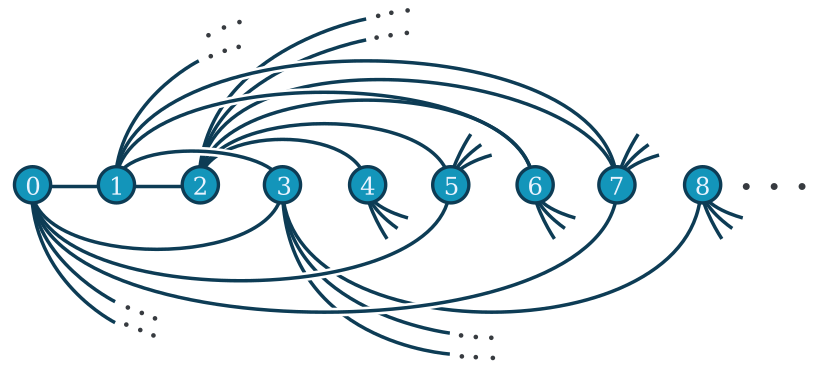
\includegraphics[scale=0.7]{Figures/Rado-graph.png}
	\caption{Binary construction of the Radó graph}
\end{figure}

\subsection{Erdös-Rényi model}
Erdös-Rényi model is the finite version of the Radó graph. In this model the parameter $p$ is usually taken as a function of $n$. This provide, unlike the past model, a variety of graphs even when $n$ tends to infinity.

\begin{defini}
Denote by $\G(n,p)$ to the probability space formed by all the graphs of $n$ vertices and probability measure 
$$ \P\Big(G\in \G(n,p)\Big) = p^{k} (1-p)^{\binom{n}{2}-k} $$
where $k$ is the number of edges in $G$, the $\sigma$-algebra is given by the power set.
\end{defini}

Note: There is a variation of the model, where we rather choose randomly exactly $m$ edges among the $\binom{n}{2}$ possible.

We can also think this model like $\binom{n}{2}$ i.i.d. $Bernoulli(p)$ that represent the edges. Using what we know about this r.v. we can immediately get some properties of the degree of a given vertex $v$.

\begin{itemize}
\item The probability that a given vertex $v$ has degree $k$ is given by
$$b(k; n-1,p) = \binom{n-1}{k} \cdot p^{k} \cdot (p-1)^{n-k-1}$$
\item The expected degree is $(n-1)\cdot p$
\item The variance of this degree is $(n-1)\cdot p \cdot (1-p)$
\end{itemize}

The degree distribution can be helpful to do optimizations in the rigid expansions algorithms. This is outlined in the next chapter.

\section{Rigid expansions}

 We will focus in the rigidity calculations for the finite case. Then, we will analyze when $n$ tends to infinite. For this, we need the calculations of the probability that the following events occur.

\begin{itemize}
\item A vertex $v$ is uniquely determined by $A_{m}$, a subset of vertices of size $m$
\item $A_k$ generate a rigid expansion
\item $A_k$ generate a rigid expansion with $s$ new elements
\end{itemize}

For the calculations concerning the first event, take a look to following picture

\begin{figure}[h!]
	\centering
	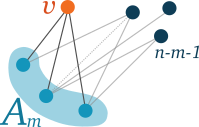
\includegraphics[scale=1]{Figures/uni.png}
	\caption{Probability of uniquely determined vertices}
\end{figure}

If $<A_{m}> = v$, there is a edge between $v$ and every vertex in $A$, and none of the remaining $n-m-1$ vertices is also connected to every vertex in $A$, i.e.
$$\P (E_m) = \P(<A_{m}> = v) = p^{m}(1-p^{m})^{n-m-1}$$
Using the \texttt{networkx} library in \texttt{python} we reproduce the following experiment:

\begin{cajita}
\textbf{Uniquely determined vertex experiment} \hfill \break
Fixing $n,p,m$.
\begin{enumerate}
\item Generate an Erdös-Rényi graph $G\in \G(n,p)$ with labeled vertices.
\item Excluding the $n$-th vertex, take a random subset of vertices of size $m$.
\item Verify if this random set uniquely determine the $n$-th vertex.
\end{enumerate}
\end{cajita}

In the next chapter we explain how to generate random graphs for the first. To simplify the process we took, without loosing generality, the last vertex as a particular element of the experiment. When $m=n$ there is no need to do the experiment.

Fixing $n$ and $p$ we computed the empiric probability for each possible value of $m$. In the following figure appear these estimates together with the theoretical calculations.

\begin{figure}[h!]
	\centering
	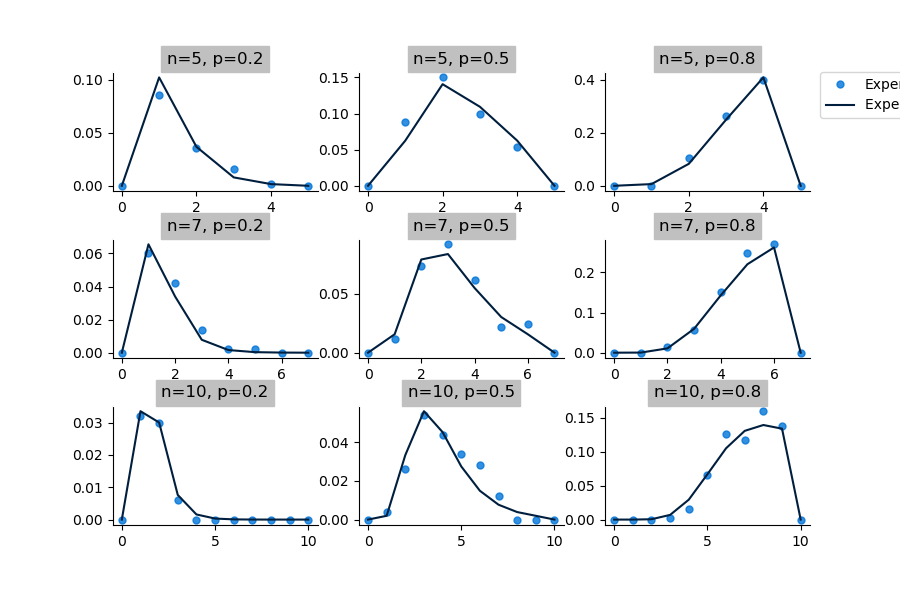
\includegraphics[scale=0.55]{Python/Figures/Uniquely-determinated-fixed-vertex.png}
	\caption{Theoretical and empirical probabilities of uniquely determined a vertex. For different values of $n$ and $p$ varying among all the possible values of $m$}
\end{figure}

For these calculations we repeated this experiment 500 times and count the number of times that the random set uniquely determine the $n$-th vertex. The empiric probability is the ratio of times when this happened.

Notice that there are certain values of $m$ more \textit{effective} than others, in the sense that, depending on the parameters of the model, it is more likely that a subset of certain size uniquely determine a vertex. This can be used, as described in the next chapter, to do optimizations in the simulations.
 
The following table is a summary of the maximum of differences between these two values for distinct values of $n$ and $p$. These values are indicators that the simulations and the calculations actually describe the same event.
\vspace{0.3cm}
\input{Python/Txt/table.txt}
\vspace{-0.3cm}
 
For the second event, if $A_k$ does not generate a rigid expansion is because none of the subsets of $A_{k}$ determined uniquely a vertex outside of it. We have:
$$\P(A_k \text{ generates a rigid expansion}) = 1 -  \prod_{m=1}^{k} (\rho_{m,k})^{\binom{k}{m}}$$
where $\rho_{m,k} = \Big(1 -  \P(E_m)\Big)^{n-k}$.

Just as before, we reproduce the following experiment:
 
\begin{cajita}
\textbf{Rigid expansion experiment} \hfill \break
Fixing $n,p,k$.
\begin{enumerate}
\item Generate an Erdös-Rényi graph $G\in \G(n,p)$.
\item Take a random subset of vertices of size $k$.
\item Verify if this set generates a rigid expansion
\end{enumerate}
\end{cajita}

Notice that the third step is a critical point in this experiment; we must verify among all the possible subsets of $A_{k}$. In the next chapter we explain how this should be done.

Again, we repeated this experiment 500 times and calculated the empiric probability that a random set generate a rigid expansion. In the following figure appear empiric and theoretical probabilities for this experiment.

\begin{figure}[h!]
	\centering
	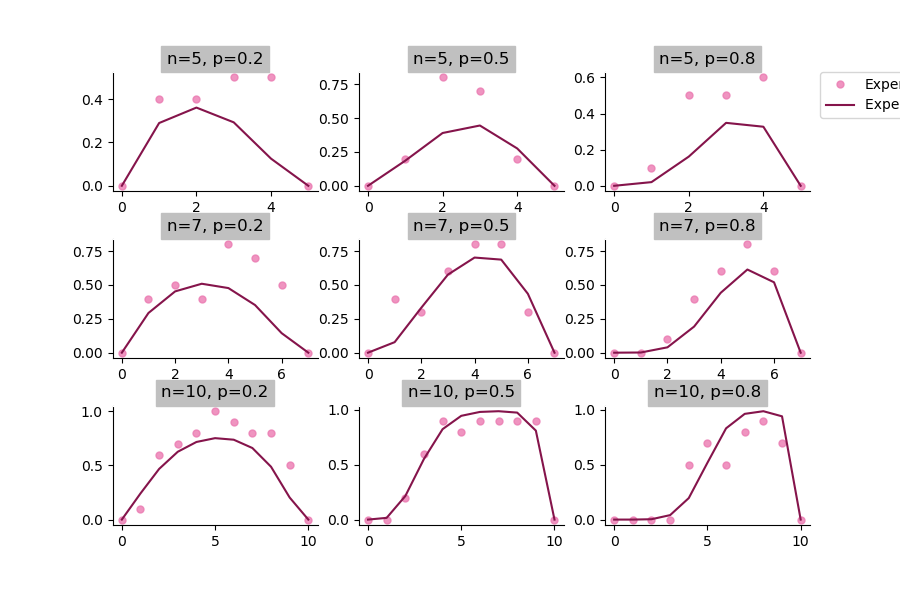
\includegraphics[scale=0.55]{Python/Figures/Expansion-probability.png}
	\caption{Theoretical and empirical probabilities of expanding $A_{k}$. For different values of $n$ and $p$ varying among all the possible values of $k$}
\end{figure}

The empirical and theoretical probabilities agree again.
 \vspace{0.3cm}
\begin{table}[htbp]
\begin{center}
\bgroup
\def\arraystretch{1.5}
\begin{tabular}{|c|c|c|c|}
\hline
n & 5 & 10 & 15 \\
\hline
 0.2 & $1e^{-8}$ & $1e^{-8}$ & $1e^{-8}$ \\\hline
 0.3 & $1e^{-8}$ & $1e^{-8}$ & $1e^{-8}$ \\\hline
 0.4 & $1e^{-8}$ & $1e^{-8}$ & $1e^{-8}$ \\\hline
\end{tabular}
\egroup
\caption{Maximums of differences between empirical and theoretical probabilities varying $m$ for different values of $n$ and $p$}
\label{tabla:sencilla}
\end{center}
\end{table}
\vspace{-0.3cm}
 
The calculations for the last question are helpful if we want to approximate the sequence of rigid expansions of $A_{k}$ by a Markov chain. Consider $\{0,1, \dots n\}$ as the states space of the Markov chain with transition matrix given by:
$$ a_{k,k+s} = \P(A_{k} \text{ generates a rigid expansion by } s \text{ elements})$$
Notice that the deterministic process stops once a iteration fails to add new vertices. In our stochastic approximation a new $G \in \G(n,p)$ is considered for each step, hence, it is allowed to \textit{"have extra tries to expand".}

This probability calculations are more difficult to obtain. To start understanding this phenomenon we can simulate with our computational tools the following experiment:
 
\begin{cajita}                                                                                                                                                                
\textbf{Increase size by a rigid expansions experiment} \hfill \break
Fixing $n,p,k$.
\begin{enumerate}
\item Generate an Erdös-Rényi graph $G\in \G(n,p)$.
\item Take a random set of vertices $A_{k}$.
\item Produce the first rigid expansion from the graph spanned by $A_{k}$
\item Return the size of the expanded subgraph
\end{enumerate}
\end{cajita}

This experiment yields a random variable which depends on $n, p$ and $k$. Fixing $n$ and $p$ we obtained a sample of size 50 for every possible value of $k$. Using the resulting histogram as an empirical density function we obtain the following figure. It graphically describes the nature of the transition matrix of a sequence of rigid expansions.

\begin{figure}[h!]
	\centering
	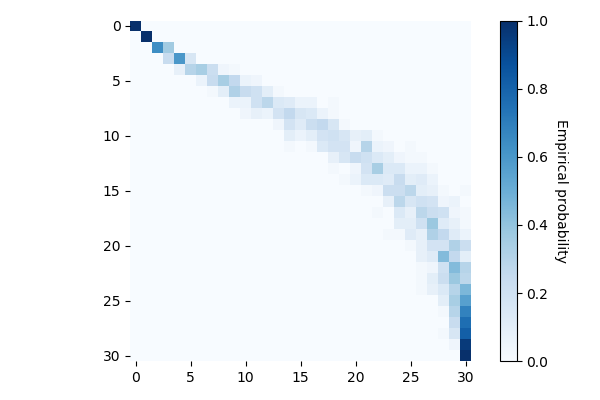
\includegraphics[scale=0.7]{Python/Figures/Transition-matrix-secuence-of-rigid-expansions.png}
	\caption{Empirical transition probability matrix}
\end{figure}

\section{Radó graph as a model for the curve graph}

In chapter one we settled the bases to model the curve graph associated to any given surface. Summarizing the results, the exposed models should, at least, guarantee the following properties:

\begin{enumerate}
\item Countably infinite number of vertices
\item Connectedness
\item Locally infinite
\item Clique number $3g-3+m$
\item Infinite diameter
\end{enumerate}

The Radó graph satisfy that every finite or countably infinite graph is an induced subgraph of it \cite{DarReferenciaAqui1}. The restriction in the clique number of $C(S)$ implies that, if $S$ is a surface of finite genus, is not possible that the Radó graph is embedded into $C(S)$. Even more, a result by by Bering and Gaster \cite{beringGaster} state that the converse is also valid.

\begin{theorem}
The random graph embeds into the curve graph $C(S)$ of a surface $S$ if and only if $S$ has infinite genus.
\end{theorem}

Therefore, if we want to study the curve graph of a surface of finite genus using the Radó graph, we have to think it as a subgraph of it. A simple but naive approach to do it is to take a random subset of vertices of a graph $G\in \G(\N, p)$ and then consider the vertex induced subgraph. It turns out that for a.e. $G\in \G(\N, p)$ the sequence $cl(G_n)$ is almost entirely determined.

\begin{theorem}
For a.e. $G \in \G(\N,p)$ there is a constant $m_0 = m_{0}(G)$ such that if $n \geq m_o$ and $n'_{r} \leq n \leq n_{r+1}$, then $cl(G_{n}) = r$.
\end{theorem}

The proof of this theorem can be find in \cite[Bollobás p.~284]{Bollobas}. The theorem states that if $r$ is fixed and finite, the number of vertices should be finite as well. Therefore, \textbf{it is not possible to obtain the curve graph by an uniform selection of vertices}. 

Notice that this property seems not generic at all, unlike the others listed above, the clique number is the only property which actually depends on the genus of the surface.

Complications like this appear often in the literature, for example in \cite{Alcazar15} they want to ensure that a random graph does not have cycles (in this case it is implied that the clique number is 2). A discrete MCMC algorithm was used to sample uniformly random trees of size $n$, with the \texttt{generate algorithm}. It produce a maximal tree of any not directed graph with $n$ vertices taken uniformly among all the possible ones. In the appendix we summarize the results of this method, for a deeper analysis look at \cite{Broder89}.

Even if we can provide an analog of the generate algorithm to ensure a fixed clique number, the idea is to study rigid expansions with a simpler probabilistic approach. In this spirit, it remains to examine the plausibility of the Erdös-Rényi model and do an asymptotic analysis.

\section{Erdös-Rényi as a model for the curve graph}

\subsection{Connectivity}
\begin{theorem}
Let $\omega(n)$ be a function that tends to infinity arbitrarily slow as $n$ tends to infinity
\begin{itemize}
\item If $p\geq \frac{log(n)+ \omega(n)}{n}$ then 
$$\lim_{n \to \infty} \P(G \in \G(n,p) \text{ is connected}) = 1$$
\item If $p\leq \frac{log(n)- \omega(n)}{n}$ then
$$\lim_{n \to \infty} \P(G \in \G(n,p) \text{ is disconnected}) = 1$$
\end{itemize}
\end{theorem}
 
This can be proven by first showing that for a large $n$ almost all graphs consists of a connected graph having $n-k$ effective vertices and $k$ isolated points, the theorem follows from a counting argument. The complete proof can be found in \cite[Erdös-Rényi, p. 59]{OnRandomGraphs}.
 
\subsection{Locally infinity}

The following theorem gives a complete description of the degree distribution; consider $X_{k} = X_{k} (G)$, the random variable that describes the number of vertices of degree $k$ in a graph $G$.

\begin{theorem}
Let $\epsilon>0$ be fixed, $\epsilon n^{-3/2} \leq p = p(n) \leq 1 - \epsilon n^{-3/2}$, let $k = k(n)$ be a natural number and set $\lambda_{k} = \lambda_{k}(n) = n\cdot b(k;n - 1,p)$. Then the following assertions hold.

\begin{itemize}
\item If $\lim \lambda_{k}(n) = 0$, then $\lim P(X_{k} = 0) = 1$. 
\item If $\lim \lambda_{k}(n) = \infty$, then $\lim P(X_{k} > t) = 1$
for every fixed $t$.
\item If $0 < \lim\lambda_{k}(n) < \lim \lambda_{k}(n) < \infty$,
then $X_{k}$ has asymptotically Poisson distribution with mean $\lambda_{k}$: 
$$P(X_{k} = r) \sim e^{\lambda_{k}}\cdot \lambda_{k}^{r}/ r!$$
for every fixed $r$.
\end{itemize}
\end{theorem}

The hypothesis on $p$ appears when we consider a loose upper bound on the expected degree of $X_ {k}$. If $pn^{2} \to \infty $ then almost every $ G \in \G (n, p) $ consist of independent edges and isolated vertices. The complete argument of this claim among with the proof of the theorem can be found in \cite[Bollobás, p.61]{Bollobas}.

If $k$ is a finite fixed number and $\lim \lambda_{k}(n) = 0$ then a.a.s there are no vertices of finite degree. In the second case there are an infinite number of vertices with degree $k$. In the third case we can describe explicitly the degree distribution, it will concentrated in a finite range around the mean $\lambda_{k}$. 

To ensure the locally infinite property using this theorem, $p = p(n)$ needs to satisfy the first case for any fixed $k$ i.e.
$$\lambda_{k} = n \binom{n-1}{k} p^{k} (1-p)^{n-k-1} \to 0$$
We can rather do a simplification of the matter using that $deg(v)$ behaves like a random binomial variable. Proposing a more simple expression for $p$ we can simplify the expressions which determine the threshold. 
\begin{theorem}\label{conectivityRCC}
Let $G \in \G(n,p)$, $\epsilon>0$ and $a>0$ be fixed, taking $p=\frac{\epsilon}{n^{a}}$ and 
\begin{itemize}
    \item If $a\geq 1$ then 
    $$\lim_{n \to \infty} \P(deg(v) \text{ is finite}) = 1$$
    \item If $a<1$ then
     $$\lim_{n \to \infty} \P(deg(v) \text{ is infinite}) = 1$$
\end{itemize}
\end{theorem}

\begin{proof}
We will assume that $a\neq 1$; when $a=1$ we know this is the Binomial's Poisson approximation. When $k=0$ we have
$$\displaystyle\lim_{n\to \infty} \P\Big(deg(v)= 0\Big) = \displaystyle\lim_{n\to \infty } \left( 1 - \frac{\epsilon}{n^a}\right)^n = \displaystyle\lim_{n\to \infty} exp\left( ln \left( 1 - \frac{\epsilon}{n^a}\right)^n\right) = \displaystyle\lim_{n\to \infty} exp\left(n \cdot ln \left( 1 - \frac{\epsilon}{n^a}\right)\right)$$
If $f(n)=  n \cdot ln \left( 1 - \frac{\epsilon}{n^a}\right)$, then $\displaystyle\lim_{n\to \infty} f(n) = \displaystyle\lim_{n\to \infty}\frac{ln \left( 1 - \frac{\epsilon}{n^a}\right)}{\frac{1}{n}}$. Using L'ôpital's rule for limits we obtain:
$$\displaystyle\lim_{n\to \infty } f(n) = 
\displaystyle\lim_{n\to \infty } \frac{\frac{1}{\left( 1 - \frac{\epsilon}{n^a}\right)}\cdot (\epsilon a n^{-a-1})}
{-1\cdot n^{-2}} = 
\displaystyle\lim_{n\to \infty } \frac{\frac{n^a}{n^{a} - \epsilon}\cdot (\epsilon a n^{-a-1}) \cdot {n^{2}}}{-1} = 
\displaystyle\lim_{n\to \infty } - \frac{\epsilon a n}{n^{a} - \epsilon} =
\displaystyle\lim_{n\to \infty } - \frac{\epsilon a}{a n^{a-1}}
$$
from here, if $a>1$ then $\displaystyle\lim_{n\to \infty } f(n) = 0$, if $a<1$ then $\displaystyle\lim_{n\to \infty } f(n) = -\infty$. So we have
$$ \displaystyle\lim_{n\to \infty} \P\Big(deg(v)=0\Big) = \begin{cases} 
\displaystyle\lim_{n\to \infty}e^{f(n)} = 1, & \mbox{if } a>1 \\ 
\displaystyle\lim_{n\to \infty}e^{f(n)} = 0, & \mbox{if } a<1 \end{cases} $$
Meaning that when $a>1$ then a.a.s the graph does not have any edges, this conclude the first part of the theorem. For $k>0$ and $a<1$:
\begin{center}
\begin{tabular}{ r l }
 $\displaystyle\lim_{n\to \infty } \P\Big(deg(v)=k\Big) =$ & $\displaystyle\lim_{n\to \infty} \binom{n}{k} \cdot \left( \frac{\epsilon}{n^a} \right)^k \cdot \left( 1-\frac{\epsilon}{n^a}\right)^{n-k}$ \\
$=$ &  $\displaystyle\lim_{n\to \infty} C_{k}\cdot n^k\cdot  \frac{\left(\frac{\epsilon}{n^a}\right)^k} {\left(\frac{n^a - \epsilon}{n^a}\right)^k} \cdot \left(1-\frac{\epsilon}{n^a}\right)^{n} $\\
$=$ &  $C_{k}\displaystyle\lim_{n\to \infty} n^k \cdot \left(\frac{1} {n^a - \epsilon}\right)^k \cdot \left(1-\frac{\epsilon}{n^a}\right)^{n} $\\
$=$ &  $C_{k} \displaystyle\lim_{n\to \infty}  n^s\cdot \left(1-\frac{\epsilon}{n^a}\right)^{n}$\\
\end{tabular}
\end{center}

where $s=k(1-a)>0$, hence $\displaystyle\lim_{n\to \infty } \P\Big(deg(v)=k\Big) = 0$

\end{proof}

\subsection{Clique number}

\begin{theorem}
Let $r = r(n) = O(n^{1/3})$ and let $p=p(n)$, $0<p<1$, be such that
$$\binom{n}{r} p^{\binom{r}{2}} \to \infty \text{ and } \binom{n}{r+1} p^{\binom{r+1}{2}} \to 0 $$
Then a.e $G\in\G(n,p)$ has clique number $r$.
\end{theorem}

The second condition on $p$ implies that almost no $G\in\G(n,p)$ contains a $K^{r+1}$ so $cl(G_{p})\leq r$ asymptotically almost surely. The first condition on $p$ is simply that $\E (X_{r}) \to  \infty$, where $X_r$ denote the random variable which counts the number of $r-$cliques in a graph $G$. This theorem can be proven using the calculations for $\E(X_{r})$ and a first moment argument. A full proof can be find in \cite[Bollobás, p.290]{Bollobas}.

Notice that in the hypothesis of the theorem $r$ is not fixed. Due that $r=3g-3+m$ this implies that the curve graph could corresponds to a surface whether of infinite diameter or with an infinite number of punctures

with the Stirling approximation for $\binom{n}{r}$ we can try to fit this result with the previous expressions.
$$E_{r} = (2\pi)^{- 1/2} n^{n+ 1/2} (n - r)^{-n+r-1/2} r^{-r-1/2} p^{r(r- 1)/2}$$
Taking $r$ as a fixed finite number we have
$$\displaystyle\lim_{n\to \infty } E_{r} = \displaystyle\lim_{n\to \infty} c_{r}\cdot \frac{n^{n+1/2}}{(n-r)^{n+1/2}} \cdot (n-r)^{r}\cdot p^{r(r-1)/2} = c_{r}\cdot \displaystyle\lim_{n\to \infty}  (n)^{r}\cdot p^{r(r-1)/2}$$
Taking $p=\epsilon/n^{a}$ as in \ref{conectivityRCC} it results in
$$\displaystyle\lim_{n\to \infty } E_{r} =  c_{r}\cdot \displaystyle\lim_{n\to \infty}  (n)^{r}\cdot\Big(\frac{1}{n^a}\Big)^{r/2}\cdo \Big(\frac{1}{n^a}\Big)^{r/2}
\cdot\frac{1}{n^a}$$



. Again, \textbf{this property interfere with the proposed model}. We can still provide an analogue of Bering and Gaster result.

\subsection{Diameter}

The diameter of a graph $G$, denoted by $diam(G)$, is the maximal distance between pairs of vertices of $G$.

For surfaces of finite genus we should had ensure infinite diameter. There are a number of theorems that state the conditions under this can be done \cite[Bollobás, p.259]{Bollobas}. Nevertheless, by the past results we must guarantee that the diameter is equal to 2, so the model match the properties of curve graphs for infinite genus surfaces.

\begin{theorem}
If $p$ is taken fixed $G(n,p)$ has diameter 2 with high probability 
\end{theorem}

\begin{proof}
Consider the random variable $X_{n}$ which is the number of vertex pairs in a graph in $\G(n,p)$ with no common neighbors. By Markov's inequality we have that
$$\P(X_{n} \geq 1)\leq \E(X_{n}) = \binom{n}{2} \cdot \P(\text{two vertices doesn't have common neighbors}) = \binom{n}{2} (1-p^{2})^{n-2}$$
which tends to zero as $n\to \infty$
\end{proof}

Although this result has a simple proof, the following theorem allows a broader type of functions to be taken, letting us refine the previous thresholds.

\begin{theorem}
Let $d$ be a fixed integer $d$, if 
$$\frac{(pn)^{d-1}}{n} \to 0 \text{ and } \frac{(pn)^{d}}{n} \to \infty $$
then, with probability approaching 1 as $n$ goes to infinity $G\in\G(n,p)$ has diameter $d$
\end{theorem}

The proof of this theorem is due to Klee and Larman and can be find in \cite{diameters}. For $d=2$ this mean that $p(n)= \frac{f(n)}{n^{1/2}}$ where $f(n)\in o(n^{1/2})$ and $f(n)\to \infty$.

Coupling with the expression for $p(n)$ in \ref{conectivityRCC}, this lead us to $a<\frac{1}{2}$



%In the first chapter we mention that 
%That's why it's worth to enunciate the following theorem which can be found in \cite[Khale, 16]{Khale}.
%\begin{theorem}
%Let $k \geq 3$ and $\epsilon > 0$ be fixed. If
%$$\left(\frac{(C_{k} + \epsilon \text{log } n} {n} \right) n^{1/k} \leq p \leq \frac{n^{-\epsilon}}{n^{1/(k+1)+\epsilon}}$$
%where $C_{3} = 3$ and $C_{k} = k/2 + 1$ for $k > 3$, then w.h.p. $X$ is rationally homotopy equivalent to a bouquet of $k$-dimensional spheres.
%\end{theorem}

%We can use the Erdös-Rényi model to obtain random simplicial complexes through clique complexes. The clique complex or flag complex $X(G)$, of a graph $G$ is the simplicial complex with all complete subgraphs of $G$ as its faces. The 1-skeleton of $X(G)$ is $G$ itself. $X(G(n, p))$ will be abbreviated by $X(n, p)$ for now on.
%The main remaining conjecture for the topology of random clique complexes is that these rational homotopy equivalences are actually homotopy equivalences.

%\begin{conje}
%The bouquet-of-spheres conjecture.
%Let $k \geq 3$ and $\epsilon > 0$ be fixed. If
%$$\frac{n^{\epsilon}}{n^{1/k}} \leq p \leq \frac{n^{-\epsilon}}{n^{1/(k+1)}}$$
%then w.h.p. $X$ is homotopy equivalent to a bouquet of $k$-spheres.
%\end{conje}